\documentclass[tikz,border=2pt]{standalone}
\usepackage{amsmath,amssymb}
\usepackage{tikz}
\usetikzlibrary{matrix}

\begin{document}
% Suppose the reals in [0,1] were listed r1, r2, r3, ...; change every diagonal digit and
% the new number differs from each r_n in its n-th digit, so it is missing from the list.
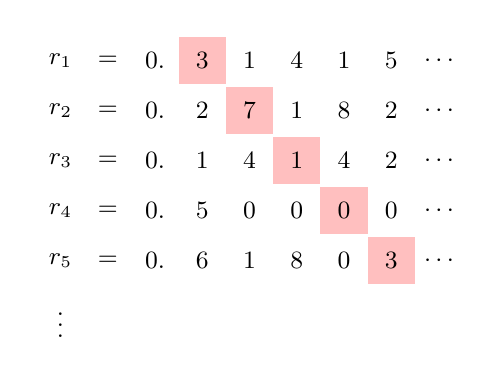
\begin{tikzpicture}[every node/.style={font=\small}]
	\matrix (M) [matrix of math nodes, nodes={minimum size=6mm, anchor=center}, column sep=0pt, row sep=1pt] at (0,0) {
		r_1 & = & 0. & |[fill=red!25]| 3 & 1 & 4 & 1 & 5 & \cdots \\
		r_2 & = & 0. & 2 & |[fill=red!25]| 7 & 1 & 8 & 2 & \cdots \\
		r_3 & = & 0. & 1 & 4 & |[fill=red!25]| 1 & 4 & 2 & \cdots \\
		r_4 & = & 0. & 5 & 0 & 0 & |[fill=red!25]| 0 & 0 & \cdots \\
		r_5 & = & 0. & 6 & 1 & 8 & 0 & |[fill=red!25]| 3 & \cdots \\
		\vdots & & & & & & & & \\
	};
\end{tikzpicture}
\end{document}
